% TeX'ing this file requires that you have AMS-LaTeX 2.0 installed
% as well as the rest of the prerequisites for REVTeX 4.0
%
% See the REVTeX 4 README file
% It also requires running BibTeX. The commands are as follows:
%
%  1)  latex apssamp.tex
%  2)  bibtex apssamp
%  3)  latex apssamp.tex
%  4)  latex apssamp.tex
%
\documentclass[prb,preprintnumbers,amsmath,amssymb, 10pt]{revtex4}
%\documentclass[preprint,showpacs,showkeys,preprintnumbers,amsmath,amssymb]{revtex4}

% Some other (several out of many) possibilities
%\documentclass[preprint,aps]{revtex4}
%\documentclass[aps, two column, amsmath,amssymb,floatfix]{revtex4}
%\documentclass[showkeys,showpacs,amsmath,amssymb,onecolumn,superscriptaddress,prl]{revtex4-1}% Physical Review B  
% \documentclass[aps,prl,reprint,showpacs,floatfix,superscriptaddress, onecolumn]{revtex4-2}

\usepackage{amsmath,amsthm,amssymb}
\usepackage{graphicx}% Include figure files
\usepackage{dcolumn}% Align table columns on decimal point
\usepackage{bm}% bold math
\usepackage{color}
\usepackage{epsfig}
\usepackage{multirow}
\usepackage{mathrsfs}
\usepackage{hyperref}
\usepackage{cleveref}
\usepackage{epstopdf}
\usepackage{subfigure}
\usepackage{autobreak}
\usepackage{tikz}

%Macros for mathematical notations

\newcommand{\V}[1]{\boldsymbol{#1}} %# vector
\newcommand{\M}[1]{\boldsymbol{#1}} %# matrix
\newcommand{\Set}[1]{\mathbb{#1}} %# set
\newcommand{\D}[1]{\Delta#1} %# \D{t} for time step size
\renewcommand{\d}[1]{\delta#1} %# \d{t} for small increment
\newcommand{\norm}[1]{\left\Vert #1\right\Vert } % norm
\newcommand{\abs}[1]{\left|#1\right|} %abs

\newcommand{\grad}{\M{\nabla}} %gradient
\newcommand{\av}[1]{\left\langle #1\right\rangle } %take average

\newcommand{\sM}[1]{\M{\mathcal{#1}}} %matrix in mathcal font
\newcommand{\dprime}{\prime\prime} % double prime
%\global\long\def\i{\iota}
%\renewcommand{\i}{\iota} %i for imaginary unit
%\renewcommand{\i}{\mathsf i} %i for imaginary unit
\newcommand{\follows}{\quad\Rightarrow\quad} %=>
\newcommand{\eqd}{\overset{d}{=}} %=^d
\newcommand{\spe}[1]{\mathscr{#1}}  %important quantities in mathscr font
\newcommand{\eps}{\epsilon}
\newcommand{\bra}[1]{\left\langle #1 \right|}
\newcommand{\ket}[1]{\left| #1 \right\rangle}
\newcommand{\braket}[2]{\left\langle #1 \middle| #2 \right\rangle}
\newcommand{\bracket}[3]{\left\langle #1 \middle| #2 \middle| #3 \right\rangle}



\begin{document}
\preprint{Preprint}

\title{Problem Formulation}
\author{Xuanzhao Gao}
% \date{}

\maketitle

\section{Model}

We consider the following simplified system:

\begin{figure*}[htbp]
    \centering
    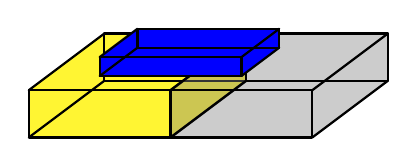
\begin{tikzpicture}[scale=1.2, line join=round, line cap=round]
      \def\s{3.0}
      \def\h{0.5}
      \def\w{1.5}

      \coordinate (I) at (0,-\h);
      \coordinate (J) at (\s - \w,-\h);
      \coordinate (K) at (\s - \w, -\h + \h);
      \coordinate (L) at (0,-\h + \h);
      \coordinate (M) at (0.8,0.6 -\h);
      \coordinate (N) at (\s+0.8 - \w,0.6 -\h);
      \coordinate (O) at (\s+0.8 - \w,0.6 -\h + \h);
      \coordinate (P) at (0.8,0.6 -\h + \h);
      % Fill faces (cube 2)
      \fill[yellow, opacity=0.8] (I)--(J)--(K)--(L)--cycle; % front
      \fill[yellow, opacity=0.8] (L)--(K)--(O)--(P)--cycle; % top
      \fill[yellow, opacity=0.8] (J)--(N)--(O)--(K)--cycle; % right side
      \draw[thick] (I)--(J)--(K)--(L)--cycle;
      \draw[thick] (M)--(N)--(O)--(P)--cycle;
      \draw[thick] (I)--(M) (J)--(N) (K)--(O) (L)--(P);

      \coordinate (I) at (\w, - \h);
      \coordinate (J) at (\s, - \h);
      \coordinate (K) at (\s, -0);
      \coordinate (L) at (\w, - 0);
      \coordinate (M) at (\w + 0.8,0.6 - \h);
      \coordinate (N) at (\s+0.8,0.6 - \h);
      \coordinate (O) at (\s+0.8,0.6 - \h + \h);
      \coordinate (P) at (\w + 0.8,0.6 - \h + \h);
      % Fill faces (cube 3)
      \fill[gray, opacity=0.4] (I)--(J)--(K)--(L)--cycle; % front
      \fill[gray, opacity=0.4] (L)--(K)--(O)--(P)--cycle; % top
      \fill[gray, opacity=0.4] (J)--(N)--(O)--(K)--cycle; % right side
      \draw[thick] (I)--(J)--(K)--(L)--cycle;
      \draw[thick] (M)--(N)--(O)--(P)--cycle;
      \draw[thick] (I)--(M) (J)--(N) (K)--(O) (L)--(P);

      % Define scale for blue cube
      \def\bluecubescale{0.5} % Adjust this value to make it smaller or larger
      \def\sblue{\s * \bluecubescale}
      \def\hblueactual{0.2} % Actual height of the blue cube, make it flatter
      \def\depthx_blue{0.8 * \bluecubescale} % Scaled x-shift for depth
      \def\depthyblue{0.6 * \bluecubescale} % Scaled y-shift for depth

      % Calculate horizontal offset to keep the blue cube centered on the base
      \pgfmathsetmacro\xoffsetblue{(\s - \sblue) / 2}

      % Calculate front-to-back offset to keep the blue cube centered on the base's top surface
      % The base's top surface depth in y-direction is 0.6 (without perspective shift)
      \pgfmathsetmacro\yoffsetbluedepth{(0.6 - \depthyblue) / 2}

      % Define coordinates for the blue cube, positioned on top of the base
      % The base's top front edge is at y=0
      \coordinate (A) at (\xoffsetblue, \yoffsetbluedepth);
      \coordinate (B) at (\xoffsetblue+\sblue, \yoffsetbluedepth);
      \coordinate (C) at (\xoffsetblue+\sblue, \yoffsetbluedepth + \hblueactual);
      \coordinate (D) at (\xoffsetblue, \yoffsetbluedepth + \hblueactual);
      % Back square (shifted) for perspective
      \coordinate (E) at (\xoffsetblue+\depthx_blue, \yoffsetbluedepth + \depthyblue);
      \coordinate (F) at (\xoffsetblue+\sblue+\depthx_blue, \yoffsetbluedepth + \depthyblue);
      \coordinate (G) at (\xoffsetblue+\sblue+\depthx_blue, \yoffsetbluedepth + \depthyblue + \hblueactual);
      \coordinate (H) at (\xoffsetblue+\depthx_blue, \yoffsetbluedepth + \depthyblue + \hblueactual);

      % Fill faces (cube 1) - now opaque
      \fill[blue] (A)--(B)--(C)--(D)--cycle; % front
      \fill[blue] (D)--(C)--(G)--(H)--cycle; % top
      \fill[blue] (B)--(F)--(G)--(C)--cycle; % right side
      % Draw faces and connecting edges
      \draw[thick] (A)--(B)--(C)--(D)--cycle;
      \draw[thick] (E)--(F)--(G)--(H)--cycle;
      \draw[thick] (A)--(E) (B)--(F) (C)--(G) (D)--(H);
    
    \end{tikzpicture}
    \caption{Illustration of the system: the bule is the material region~$\Omega_m$, the yellow and gray regions are dielectric materials:~$\Omega_1$ and~$\Omega_2$, respectively, non-filled regions are vacuum denoted as~$\Omega_0$.}
    \label{fig:system}
\end{figure*}
\noindent where the system we are interested in is the blue region, and the yellow and gray regions are dielectric materials with different permittivities.
The dielectric permittivity is then defined as a function of position:
\begin{equation}
    \epsilon(\mathbf{x}) = \begin{cases}
        \epsilon_m, & \mathbf{x} \in \Omega_m \\
        \epsilon_1, & \mathbf{x} \in \Omega_1 \\
        \epsilon_2, & \mathbf{x} \in \Omega_2 \\
        \epsilon_0 = 1, & \mathbf{x} \in \Omega_0
    \end{cases}
\end{equation}

% We formulate the problem as calculating the four-index integral~\cite{cramer2013essentials} of the form:
Our goal is to compute the following four-index integral~\cite{cramer2013essentials}:
\begin{equation}
    \begin{split}
    V_{ijkl} &= \iint \varphi_i(\mathbf{x}_1) \varphi_j^*(\mathbf{x}_1) K(\mathbf{x}_1, \mathbf{x}_2) \varphi_k(\mathbf{x}_2) \varphi_l^*(\mathbf{x}_2) \mathrm{d}\mathbf{x}_1 \mathrm{d}\mathbf{x}_2\\
    & = \int \rho_{ij}(\mathbf{x}_1) \phi_{kl}(\mathbf{x}_1) \mathrm{d}\mathbf{x}_1,
    \end{split}
\end{equation}
where~$\varphi_i(\mathbf{x})$ are the basis functions (orbitals), with a typical number of 20000,~$\rho_{ij}(\mathbf{x}) = \varphi_i(\mathbf{x}) \varphi_j^*(\mathbf{x})$ is the density distribution (may further be simplified as delta-like functions), and $\phi_{kl}(\mathbf{x})$ is the solution to the Poisson equation:
\begin{equation}\label{eq:poisson-origin}
    \grad_{\mathbf{x}} \cdot \left( \epsilon(\mathbf{x}) \grad_{\mathbf{x}} \phi_{kl}(\mathbf{x}) \right) = - \rho_{kl}(\mathbf{x}).
\end{equation}
We further assume that all density distributions are located inside the interested blue region, so that $\mathbf{x}_0 \in \Omega_I$.
Then Eq.~\eqref{eq:poisson-origin} can be rewritten as the following boundary value problem (indices omitted for simplicity):
\begin{equation}
    \begin{cases}
        \epsilon_I \Delta_{\mathbf{x}} \phi(\mathbf{x}) = - \rho(\mathbf{x})~, & \mathbf{x} \in \Omega_m \\
        \Delta_{\mathbf{x}} \phi(\mathbf{x}) = 0~, & \mathbf{x} \in \Omega_0 \cup \Omega_1 \cup \Omega_2 \\
        \phi(\mathbf{x})\mid_{\partial \Omega_i} = \phi(\mathbf{x})\mid_{\partial \Omega_j}~, & \mathbf{x} \in \partial \Omega_i \cap \partial \Omega_j \\
        \epsilon_i \mathbf{n} \cdot \grad_{\mathbf{x}} \phi(\mathbf{x})\mid_{\partial \Omega_i} = \epsilon_j \mathbf{n} \cdot \grad_{\mathbf{x}} \phi(\mathbf{x})\mid_{\partial \Omega_j}~, & \mathbf{x} \in \partial \Omega_i \cap \partial \Omega_j \\
        \phi(\mathbf{x}) \to 0~, & \abs{\mathbf{x}} \to + \infty \\
    \end{cases}
\end{equation}
where the first and second equations are for the region with or without source, the third and fifth are the boundary conditions at the interfaces between different regions, and the last one is the infinite boundary condition.
Here, $\mathbf{n}$ denotes the unit outward normal on the interface.
By solving the above system, we can obtain the potential $\phi_{kl}(\mathbf{x})$, and then by integrating over the density distribution~$\rho_{ij}(\mathbf{x})$, we can obtain the four-index integral $V_{ijkl}$.

% Specially, if the dielectric material in~$\Omega_1$ or~$\Omega_2$ can be treated as a perfect conductor, we have $\epsilon_m \to \infty$, and the equations becomes:
% \begin{equation}\label{eq:poisson-perfect-conductor}
%     \begin{cases}
%         \epsilon_0 \grad^2_{\mathbf{x}} \phi(\mathbf{x}) = - \rho(\mathbf{x})~, & \mathbf{x} \in \Omega_0 \\
%         \phi(\mathbf{x}) = 0~, & \mathbf{x} \in \Omega_1 \\
%         \phi(\mathbf{x}) = 0~, & \mathbf{x} \in \Omega_2 \\
%         % \mathbf{n} \times \grad_{\mathbf{x}} \phi(\mathbf{x})\mid_{\partial \Omega_m} = 0~, & \mathbf{x} \in \partial \Omega_m \\
%         \phi(\mathbf{x})\mid_{\partial \Omega_i} = \phi(\mathbf{x})\mid_{\partial \Omega_0}~, & \mathbf{x} \in \partial \Omega_i \cap \partial \Omega_0 \\
%         \epsilon_i \mathbf{n} \cdot \grad_{\mathbf{x}} \phi(\mathbf{x})\mid_{\partial \Omega_i} = \epsilon_0 \mathbf{n} \cdot \grad_{\mathbf{x}} \phi(\mathbf{x})\mid_{\partial \Omega_0}~, & \mathbf{x} \in \partial \Omega_i \cap \partial \Omega_0 \\
%         \phi(\mathbf{x}) \to 0~, & \abs{\mathbf{x}} \to + \infty \\
%     \end{cases}
% \end{equation}
% where the third and fourth equations enforce the perfect‑conductor conditions: the potential is zero inside the metal, and the field is normal to the surface.

\section{Solver}

In this section, we describe a boundary integral equation for the potential~$\phi(\mathbf{x})$ with a single layer potential~$\mathbf{\sigma}(\mathbf{x})$ on the boundaries.
The model is illustrated as follows:
\begin{figure*}[htbp]
    \centering
    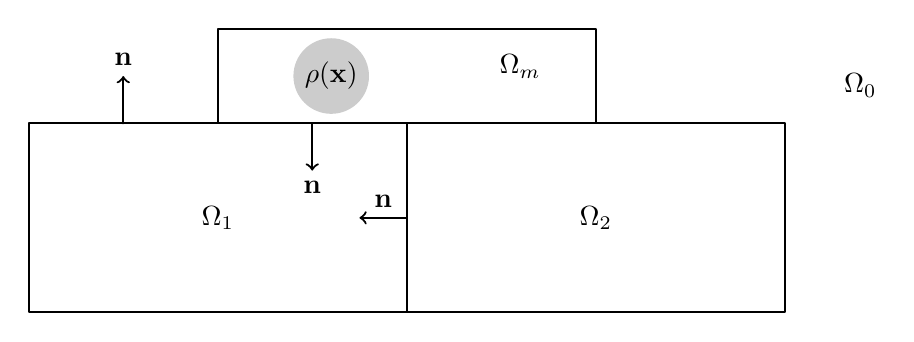
\begin{tikzpicture}[scale=1.2, line join=round, line cap=round]
      \def\s{4.0}
      \def\h{2.0}

      % Front square
      \coordinate (A) at (0,0);
      \coordinate (B) at (\s,0);
      \coordinate (C) at (\s,\h);
      \coordinate (D) at (0,\h);
      % Back square (shifted)
      \coordinate (E) at (\s, 0);
      \coordinate (F) at (2 * \s, 0);
      \coordinate (G) at (2 * \s, \h);
      \coordinate (H) at (\s, \h);

      \coordinate (I) at (0.5 * \s, 1.5 * \h);
      \coordinate (J) at (1.5 * \s, 1.5 * \h);
      \coordinate (K) at (1.5 * \s, \h);
      \coordinate (L) at (0.5 * \s, \h);
      % Fill faces (cube 1)
      % Draw faces and connecting edges
      \draw[thick] (A)--(B)--(C)--(D)--cycle;
      \draw[thick] (E)--(F)--(G)--(H)--cycle;
      \draw[thick] (I)--(J)--(K)--(L)--cycle;

      \coordinate (RI) at (1.3 * \s, 1.3 * \h);
      \coordinate (R0) at (2.2*\s, 1.2*\h);
      \coordinate (R1) at (\s / 2, \h / 2);
      \coordinate (R2) at (1.5 * \s, \h / 2);

      \node at (RI) {$\Omega_m$};
      \node at (R1) {$\Omega_1$};
      \node at (R2) {$\Omega_2$};
      \node at (R0) {$\Omega_0$};

      \coordinate (S) at (0.8*\s, 1.25*\h);
      \fill[gray, opacity=0.4] (S) circle (0.2 * \h);
      \node at (S) {$\rho(\mathbf{x})$};

      \draw[->, thick] (\s / 4, \h) -- (\s / 4, \h + 0.5) node[right, above] {$\mathbf{n}$};
      \draw[->, thick] (\s, \h / 2) -- (\s - 0.5, \h / 2) node[midway, above] {$\mathbf{n}$};
      \draw[->, thick] (\s * 3 / 4, \h) -- (\s * 3 / 4, \h - 0.5) node[right, below] {$\mathbf{n}$};
    
    \end{tikzpicture}
    % \caption{Illustration of the system: the bule and not filled region are vacuum denoted as~$\Omega_0$, the yellow and gray regions are dielectric materials:~$\Omega_1$ and~$\Omega_2$, respectively.}
    % \label{fig:2d-system}
\end{figure*}

\noindent where the gray region represents the density distribution~$\rho(\mathbf{x})$, and the arrows represent the normal direction of the boundaries (pointing from region with higher index to that with lower index).
The potential~$\phi(\mathbf{x})$ is separated into two parts:
\begin{equation}
    \phi(\mathbf{x}) = u(\mathbf{x}) + u_{\text{inc}}(\mathbf{x}),
\end{equation}
where~$u(\mathbf{x})$ is the scattered potential, and~$u_{\text{inc}}(\mathbf{x})$ is the incident potential.
The incident potential satisfies:
\begin{equation}
    \begin{cases}
    \epsilon_m \Delta u_{\text{inc}}(\mathbf{x}) = - \rho(\mathbf{x}), & \mathbf{x} \in \mathbb{R}^3 \\
    u_{\text{inc}}(\mathbf{x}) \to 0, & \abs{\mathbf{x}} \to + \infty 
    \end{cases}
\end{equation}
which is given by the following integral:
\begin{equation}
    u_{\text{inc}}(\mathbf{x}) = \frac{1}{4 \pi \epsilon_m} \int \frac{\rho(\mathbf{x}')}{|\mathbf{x} - \mathbf{x}'|} \mathrm{d}\mathbf{x}'\;.
\end{equation}
Then the scattered potential satisfies:
\begin{equation}\label{eq:scattered-potential-boundary}
    \begin{cases}
    \Delta u(\mathbf{x}) = 0, & \mathbf{x} \in \Omega_i \\
    \epsilon_i \partial_{\mathbf{n}} \left( u^+(\mathbf{x}) + u_{\text{inc}}(\mathbf{x}) \right) = \epsilon_j \partial_{\mathbf{n}} \left( u^-(\mathbf{x}) + u_{\text{inc}}(\mathbf{x}) \right), & \mathbf{x} \in \partial \Omega_i \cap \partial \Omega_j \\
    u(\mathbf{x}) \to 0, & \abs{\mathbf{x}} \to + \infty 
    \end{cases}
\end{equation}
which is a piecewise continuous function in each region.

Under the single layer potential representation, the scattered potential is given by
\begin{equation}
    u(\mathbf{x}) = \frac{1}{4 \pi} \int_{\Gamma} \frac{\mathbf{\sigma}(\mathbf{x}')}{|\mathbf{x} - \mathbf{x}'|} \mathrm{d}S(\mathbf{x}'),
\end{equation}
where~$\Gamma$ is all boundaries in the system.
Due to the existence of the single layer potential, the normal component of the scattered potential is given by
\begin{equation}\label{eq:scattered-potential}
    \begin{split}
    \partial_{\mathbf{n}} u(\mathbf{r^+}) &= \frac{1}{4 \pi} \mathbf{n} \cdot \int \grad_{\mathbf{x}} \frac{\mathbf{\sigma}(\mathbf{x}')}{|\mathbf{x} - \mathbf{x}'|} \mathrm{d}S(\mathbf{x}') - \frac{\sigma(\mathbf{x})}{2}, = D^T \mathbf{\sigma}(\mathbf{x}) - \frac{\sigma(\mathbf{x})}{2} \\
    \partial_{\mathbf{n}} u(\mathbf{r^-}) &= \frac{1}{4 \pi} \mathbf{n} \cdot \int \grad_{\mathbf{x}} \frac{\mathbf{\sigma}(\mathbf{x}')}{|\mathbf{x} - \mathbf{x}'|} \mathrm{d}S(\mathbf{x}') + \frac{\sigma(\mathbf{x})}{2} = D^T \mathbf{\sigma}(\mathbf{x}) + \frac{\sigma(\mathbf{x})}{2},
    \end{split}
\end{equation}
where $D^T$ represents the integral operator $\int_{\Gamma} \grad_{\mathbf{x}} \frac{\mathrm{d}S(\mathbf{x}')}{|\mathbf{x} - \mathbf{x}'|}$.
Then the first and third equations of Eq.~\eqref{eq:scattered-potential-boundary} are automatically satisfied, and the second equation can be rewritten as
\begin{equation}
    \epsilon_i \left( D^T \mathbf{\sigma}(\mathbf{x}) - \frac{\sigma(\mathbf{x})}{2} + \partial_{\mathbf{n}} u_{\text{inc}}(\mathbf{x}) \right) = \epsilon_j \left( D^T \mathbf{\sigma}(\mathbf{x}) + \frac{\sigma(\mathbf{x})}{2} + \partial_{\mathbf{n}} u_{\text{inc}}(\mathbf{x}) \right),~\mathbf{x} \in \partial \Omega_i \cap \partial \Omega_j.
\end{equation}
or equivalently,
\begin{equation}
    \frac{1}{2} \frac{\epsilon_i + \epsilon_j}{\epsilon_i - \epsilon_j} \sigma(\mathbf{x}) + D^T \sigma(\mathbf{x}) = - \partial_{\mathbf{n}} u_{\text{inc}}(\mathbf{x}),~\mathbf{x} \in \partial \Omega_i \cap \partial \Omega_j.
\end{equation}
By discretizing the three boundaries, the above equation can be written as a linear system of equations and solved iteratively.

% \section{Question}

% A few further questions to discuss:
% \begin{itemize}
%     \item[1.] Current model leads to edge and corner singularities. Consider that the system is at an atomic scale, is sharp edges and corners realistic?
%     % \item[2.] It seems to be more natural to consider~$\Omega_1$ and~$\Omega_2$ are semi-infinite half-spaces.
%     \item[2.] How energy band is defined in this model, if it is finite size and non-transparent in some directions?
% \end{itemize}

% I have a few questions about the model:
% \begin{itemize}
%     \item[1.] What device are we modeling? What are its dimensions, and how many orbitals are included in the calculation?
%     \item[2.] Can the dielectric materials be treated as perfect conductors? Will there be any voltage applied to them?
%     \item[3.] Where are the orbitals located? Are they confined to the center of the red cube, or can they be placed at the cube corners?
% \end{itemize}


% \bibliographystyle{apsrev}
\bibliography{ref}

\end{document}